This section shows the results obtained with the TRITIUM-Aveiro 0 prototype during its installation in Aveiro and Extremadura laboratories. The design of this prototype is shown in section \ref{subsec:TritiumAveiro}.

This prototype was first installed in the DRIM laboratory, at the University of Aveiro, where the first measurements was taken. These measurements were used to find and solve the problems, learn about low energy detection and develop a functional scintillation prototype for TRITIUM. 

First, the energy distribution of a single photon was measured from the self-emission of PMTs (dark current). To avoid the environmental light detection, the TRITIUM-Aveiro prototype was removed and the measurement was carried out only with the PMTs, the windows of which were covered with black caps. The output signals of the PMTs were digitalized, shaped and pulse-height measured by a CAEN V1724 digitalizer \cite{CAENV1724}.

The single-photon energy distribution of both PMTs is shown in Figure \ref{fig:SinglePhotonEnergyDistribution} in which a gaussian function was fitted. Due to the electrical noise of the PMT, an extrapolation (dashed line) was needed to be applied.

\begin{figure}[h]
\centering
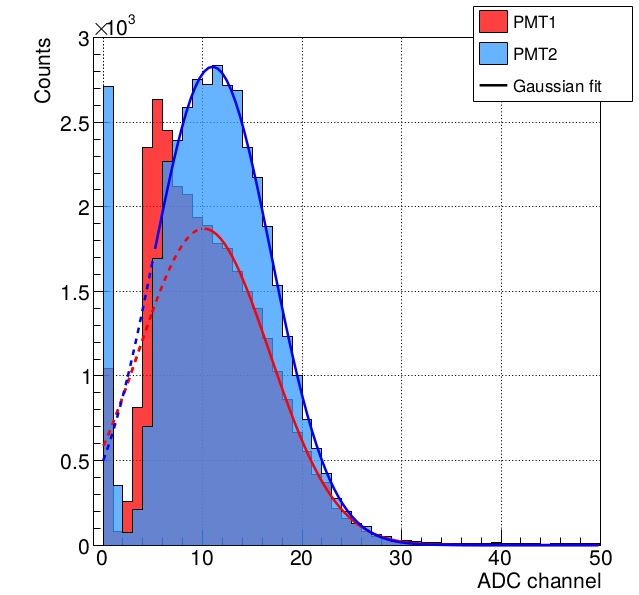
\includegraphics[scale=0.45]{7ExperimentalResultsDetectors/71ExperimentalResultsLaboratory/713TRITIUMAVEIRO0/SinglePhotonEnergyDistribution.png}
\caption{The single-photon energy distribution of both PMTs used in the TRITIUM-Aveiro 0 prototype and their sum \cite{ExperimentalPaperCarlos}.\label{fig:SinglePhotonEnergyDistribution}}
\end{figure}

As can be seen, the distribution obtained with PMT1 deviates from the Gaussian function due to the higher noise in the low energy channels. This fact indicates that it could be interesting to use PMT with very low background for future prototypes.

As DRIM laboratory was not equipped to work with liquid radioactive source such as tritiated water, the first measurements were taken with a $\ce{^{55}Fe}$ radioactive source since the energy of its $\gamma$ emission, $5.9~\keV$, is very close to the energy of tritium electrons. To do so, the TRITIUM-Aveiro 0 prototype was coupled to both PMTs using optical grease and, due to its low mean free path in solid materials, the radioactive source was placed inside the teflon vessel. This prototype was not filled with water because of the presence of the radioactive source. This measurement is shown in Figure \ref{fig:55FeMeasurement}.

\begin{figure}[htbp]
\centering
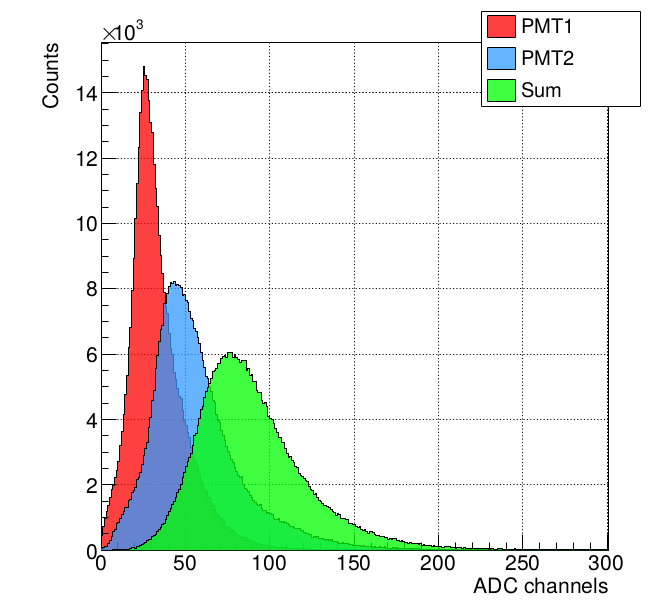
\includegraphics[scale=0.45]{7ExperimentalResultsDetectors/71ExperimentalResultsLaboratory/713TRITIUMAVEIRO0/55FeMeasurement.png}
\caption{Measurement of a $\ce{^{55}Fe}$ radioactive source with the TRITIUM-Aveiro 0 prototype \cite{ExperimentalPaperCarlos}.\label{fig:55FeMeasurement}}
\end{figure}

A shift to the right side is observed for the PMT2 data, which is produced because this PMT has a higher gain and the radioactive source was placed closer to it, reducing the attenuation of the photons.

Lastly, a passive shield test was performed in the DRIM laboratory to quantify the attenuation of the background produced by lead. To do so, the $\ce{^{55}Fe}$ radioactive source was removed and the electronical chain explained in appendix \ref{App:ElectronicSystemAveiro} was used in counting mode for this test.

The measurements, shown in Figure \ref{fig:LeadShieldTest}, were carried out in three different situations. The first, region A, in which the measurement was performed without using any lead foil, the second, region B, in which lead foil with a thickness of $2.5~\mm$ was used and the third, region C, in which another lead foil layer with the same thickness (total thickness of $5~\mm$) was used.

\begin{figure}[htbp]
\centering
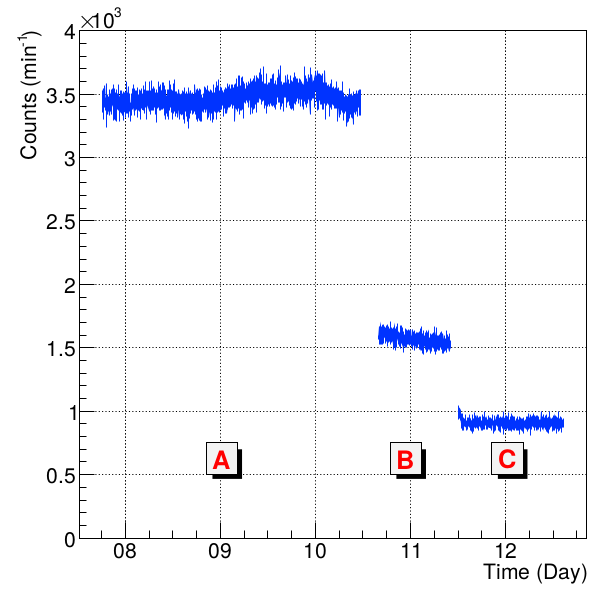
\includegraphics[scale=0.4]{7ExperimentalResultsDetectors/71ExperimentalResultsLaboratory/713TRITIUMAVEIRO0/LeadShieldTest.png}
\caption{Measurement of the background with TRITIUM-Aveiro 0 prototype covered with different thicknesses of lead \cite{ExperimentalPaperCarlos}.\label{fig:LeadShieldTest}}
\end{figure}

As can be seen, in the region A, the average of the data adquired during $2.5$ days is $3.5 \cdot{} 10^3$ counts/min ($58$ counts/sec). In the region B a reduction of more than two times was observed, measuring an average of $1.6 \cdot{} 10^3$ counts/min ($26$ counts/sec). In the region C a reduction of about 4 times relatively to the region A is observed, measuring an average of $0.9 \cdot{} 10^3$ counts/min ($15$ counts/sec).

It has to be taken into account that the case C is the real situation that is present in Arrocampo since, as it has been shown in section \ref{subsec:SetUpActiveShield}, the thickness of the lead shielding ise $5~\mm$.

As it was said, the DRIM laboratory was not equipped to work with a liquid radioactive source such as tritiated water, so this prototype was installed in the LARUEX laboratory, at the University of Extremadura to finalize with the characterization measurements. 

First, the background of the prototype was measured during 4 days. For this task, the prototype was filled with ultrapure water and covered with lead bricks with a thickness of XXX. The time of each measurement is $1$ minut and the data is shown in Figure \ref{subfig:MeasurementInRealTime} and \ref{subfig:DistributionofMeasurement} in which a gaussian fit was done. 

\begin{figure}
\centering
    \begin{subfigure}[b]{0.45\textwidth}
    \centering
    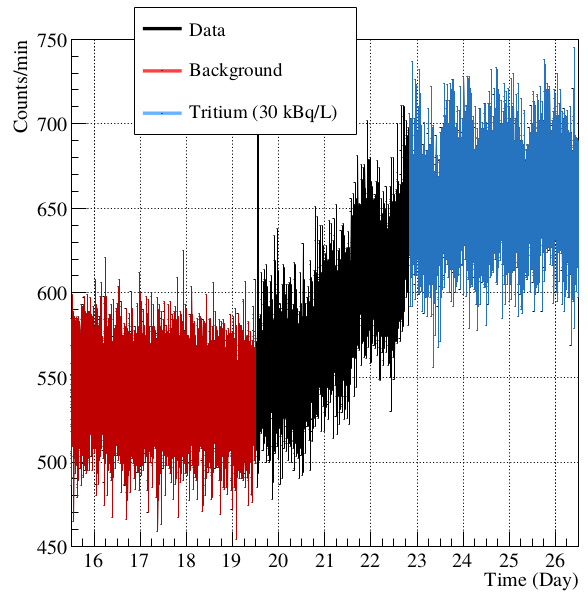
\includegraphics[width=\textwidth]{7ExperimentalResultsDetectors/71ExperimentalResultsLaboratory/713TRITIUMAVEIRO0/Tritium_1min.png}  
    \caption{Counts per minut measured as a function of time.\label{subfig:MeasurementInRealTime}}
    \end{subfigure}
    \hfill
    \begin{subfigure}[b]{0.45\textwidth}
    \centering
    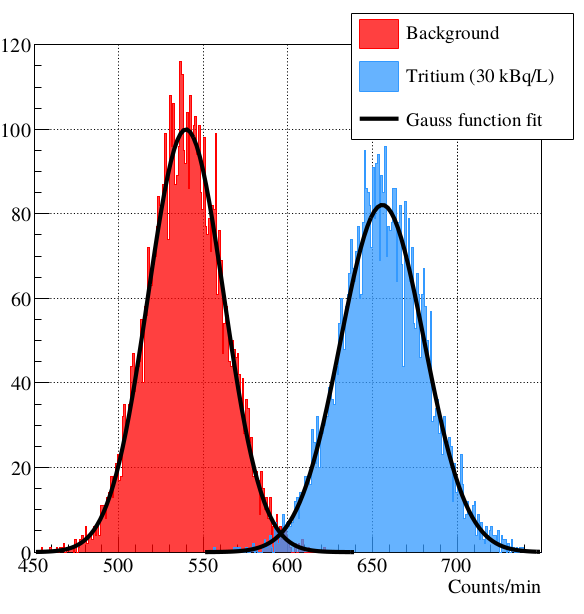
\includegraphics[width=\textwidth]{7ExperimentalResultsDetectors/71ExperimentalResultsLaboratory/713TRITIUMAVEIRO0/Tritium_Gaus_1_min.png}  
    \caption{Distribution of the acquired data.\label{subfig:DistributionofMeasurement}}
    \end{subfigure}
 \caption{Measurements of the background and tritium liquid source (with an activity of $29.8~\kilo\becquerel/\liter$) performed with the TRITIUM-Aveiro 0 prototype and integred during a minute \cite{ExperimentalPaperCarlos}.}
 \label{fig:BackgroundTritium1min}
\end{figure}

As a result of the gaussian fit, an average ($N_B$) of $540$ counts/min and standard deviation ($\sigma_{Nb}$) of $22.61$ counts/min was obtained. To calculate the Minimum Detectable Activity (MDA), the detection limit concepts developed by Lloyd A. Currie \cite{CurieLimit} was applied.  With this concepts, the minimum net counts with the probability of a false-negative less than a $5\%$, $N_D$, and minimum net currents with the probability of a false-positive less than a $5\%$, $L_C$, called critical level, are calculated using the equations:

\begin{equation}
L_C = 2\kappa\sigma_{Nb} =53 ~\text{counts/min}
\label{eq:EquationCriticalLimit}
\end{equation}
\begin{equation}
L_D = \kappa^2 + 2L_C = 108~\text{counts/min}
\label{eq:EquationNetCounts}
\end{equation}

Both values refer to the net counts per minute after background subtraction, so, $L_C'$ and $N_D'$ refered to the detector signal (before background subtraction) are $593$ and $648$ counts/min respectively.

To find the MDA associated to this $N_D'$, tritiated water was slowly added  so that the tritium water activity increased continuously up to an average of $656 \pm 0.43$ counts/min. Then, the activity of this solution was measured with a Quantulus system, obtaining a MDA of $29.8~\kilo\becquerel/\liter$.

The tritium detection efficiency can be calculated from the quotient of the net tritium counts per second measured, $1.93 \pm 0.58$ counts/sec, and the activity of the tritium source used. The efficiency obtained is $(6.49 \pm 1.94)\cdot{} 10^{-2}~ \frac{\text{c}/\second}{\kilo\becquerel/\liter}$.  The value obtained with TRITIUM-Aveiro 0 prototype is larger than the efficiency reported by other similar experiments, Table \ref{tab:PlasticScinTritium}. This is also larger than the efficiency obtained with previous TRITIUM prototypes, an expected result since the active area of this prototype is on order of magnitud larger.

The specific efficiency is calculated to compare with other scintillating detectors, the value of which is $(1.59 \pm 0.48)\cdot{} 10^{-5}~ \frac{\text{c}/\second}{\kilo\becquerel/\liter}\frac{1}{\cm^{2}}$. Comparing with the specific efficiency obtained with scintillating detectors developed in other experiments, Table \ref{tab:PlasticScinTritium}, the value obtained for TRITIUM-Aveiro 0 prototype is close the largest specific efficiency, obtained by Hofstetter. However this prototype has a worsen specific efficiency than other prototypes developed in TRITIUM experiment such us TRITIUM-IFIC 1. A possible reason is that the fibers used in this prototype are not polished or cleaned. Therefore, the importance of the fiber polishing and cleaning process is again exhibed.

It can also be noted that the efficiency uncertainties obtained for this prototype are greater than those obtained in the previous TRITIUM prototypes. The reason of that is a difference in the measurement time. The measurement time used for the TRITIUM-Aveiro prototype is $1$ minute, while that used for the previous prototypes is $10$ minutes. Smaller uncertainties are achieved in the measured counts and, therefore, in the efficiency when longer measurements are taken.

Finally, as lower uncertainties in the measured counts allow a lower MDA to be achieved, longer measurements are studied to quantify the reduction of the MDA of this prototype. For this task, groups of 60 successive measurements are integred, resulting in several measurements of 60 minutes. The adquired data is shown in Figure \ref{fig:Tritium60min}, where it can be checked a smaller relative uncertainty than the values for $1$ minute.

\begin{figure}[h]
\centering
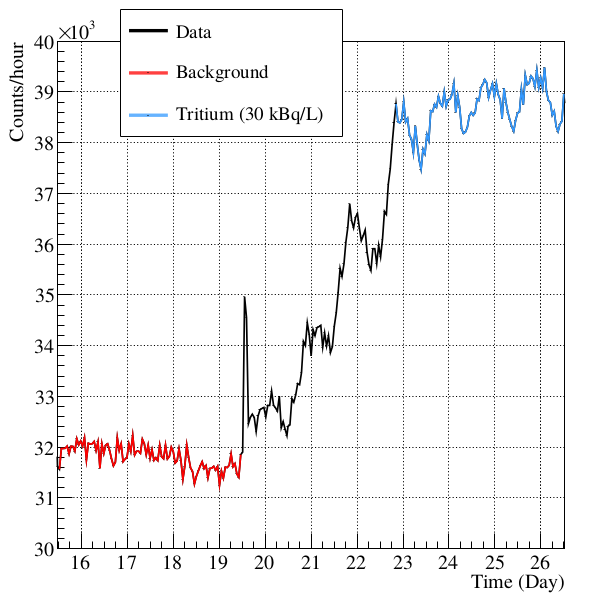
\includegraphics[scale=0.45]{7ExperimentalResultsDetectors/71ExperimentalResultsLaboratory/713TRITIUMAVEIRO0/Tritium_60min.png}
\caption{Measurements of the background and tritium liquid source (with an activity of $29.8~\kilo\becquerel/\liter$) performed with the TRITIUM-Aveiro 0 prototype and integred during an hour \cite{ExperimentalPaperCarlos}.\label{fig:Tritium60min}}
\end{figure}

In this case, the average and uncertainty of the measured background data are $3.186 \cdot{} 10^{4}$ and $228$ counts per hour respectively. Using the equations \ref{eq:EquationCriticalLimit} and \ref{eq:EquationNetCounts}, the values of $L_C=530$ and $N_D=1043$ counts per hour are obtained respectively. Assuming linearity between the measured counts for the background and the tritiated water, $3.872\cdot{}10^4$ counts per hour, this $N_D$ correspons of a MDA of $4.53~\kilo\becquerel/\liter$.

A diarly oscilation is clearly observed in the Figure \ref{fig:Tritium60min}, showing that the measurements are affected by external light. This oscilation begins on the $19^{th}$ day, where the water closed circuit pump was installed, so it is likely that the light leak is produced through this system.







%para explicar las señales de la electrónica utilizar la presentación situada en: 
%/media/marcosmr/ALMACEN/documents/doctorado/Conferencias/Meetings_TRITIUM/MERIDA-18-09-2018
